\chapter{Design and Implementation}\label{system-architecture}

\minitoc

In this chapter, we explore VV's design and implementation, detailing the architecture's modular framework and its components' interplay. It emphasizes the principles of modularity, extensibility, and object-oriented design, showcasing how these foundational elements combine to a versatile, scalable system.

\section{High-level Architecture}\label{high-level-architecture}

To facilitate a comprehensive understanding of the
system\textquotesingle s architecture, this section presents a
high-level overview of the primary classes and their interactions.
Figure \ref{fig:class_diag1} below provides a simplified visual representation of the class
structure and their relationships. It\textquotesingle s important to
note that this diagram is an abstraction intended to clarify the core
architectural elements; it does not depict every attribute or method
within these classes. The diagram has been constructed using PlantUML
\cite{48}.

\begin{figure}[ht]
  \centering
  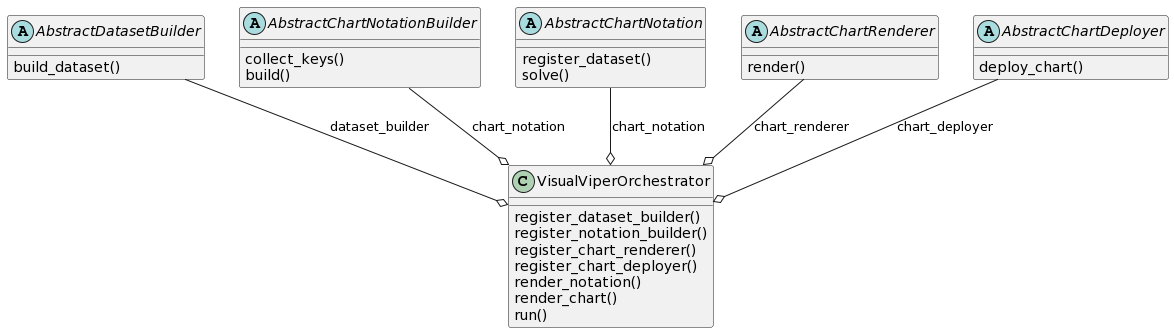
\includegraphics[width=\textwidth]{media/fig8.png}
  \caption{High-level Class Diagram of System Architecture.}
  \label{fig:class_diag1}
\end{figure}

The architecture of the VV system is designed to be both modular and
extensible, adhering to the principles of OOP. This design allows for
high cohesion among components, low coupling between modules, and
promotes scalability. To elaborate on the components that constitute
this architecture, we have categorized them into Abstract Classes,
Concrete Implementations, and an Orchestrator Class.

\subsection{Key Classes and
Components}\label{key-classes-and-components}

The Abstract Classes act as templates or interfaces, specifying what
actions must be performed but not how to perform them. Concrete
Implementations are subclasses that provide the specific
\textquotesingle how-to\textquotesingle, the logic and the behavior. The
Orchestrator Class serves as the orchestrating agent that ties these
different components together into a cohesive, functioning system.

\paragraph{Abstract Classes}\label{abstract-classes}

\begin{itemize}
\item
  \textbf{AbstractDatasetBuilder}: Provides the framework for
  constructing datasets.
\item
  \textbf{AbstractChartNotation}: Functions as the foundational class
  for handling chart notations. It provides the methods for registering
  datasets and solving elements.
\item
  \textbf{AbstractChartRenderer}: Serves as the interface for chart
  rendering mechanisms.
\item
  \textbf{AbstractChartDeployer}: Serves as the base class for all chart
  deployment mechanisms.
\end{itemize}

\paragraph{Concrete Implementations}\label{concrete-implementations}

\begin{itemize}
\item
  \textbf{GoogleSpreadsheetDatasetBuilder}: Specially designed to build
  datasets from Google Spreadsheets.
\item
  \textbf{AltairChartRenderer}: A concrete implementation of
  AbstractChartRenderer, which specifically uses Vega-Altair for
  rendering charts \cite{49}.
\item
  \textbf{GdriveChartDeployer} and \textbf{MiroChartDeployer}: These are
  specialized implementations of AbstractChartDeployer designed to
  deploy charts on Google Drive and Miro, respectively.
\end{itemize}

\paragraph{Orchestrator Class}\label{orchestrator-class}

\begin{itemize}
\item
  \textbf{VisualViperOrchestrator}: This class manages the interaction
  between the various components. It references a DatasetBuilder, a
  ChartNotationBuilder, a ChartRenderer, and a ChartDeployer. This
  allows the orchestrator to manage the flow of operations.
\end{itemize}

\subsection{Component Interactions}\label{component-interactions}

The VisualViperOrchestrator serves as the fulcrum around which the
entire architecture revolves. It dynamically links to various
components, directing the flow of data and operations throughout the
system. Subclasses of AbstractDatasetBuilder,
AbstractChartNotationBuilder, AbstractChartRenderer, and
AbstractChartDeployer, can be plugged into the orchestrator, thereby
fulfilling the design goals of modularity and extensibility.

\afterpage{%
  \clearpage% To flush out all floats, might not be what you want
  \begin{landscape}
\begin{figure}[ht]
  \centering
  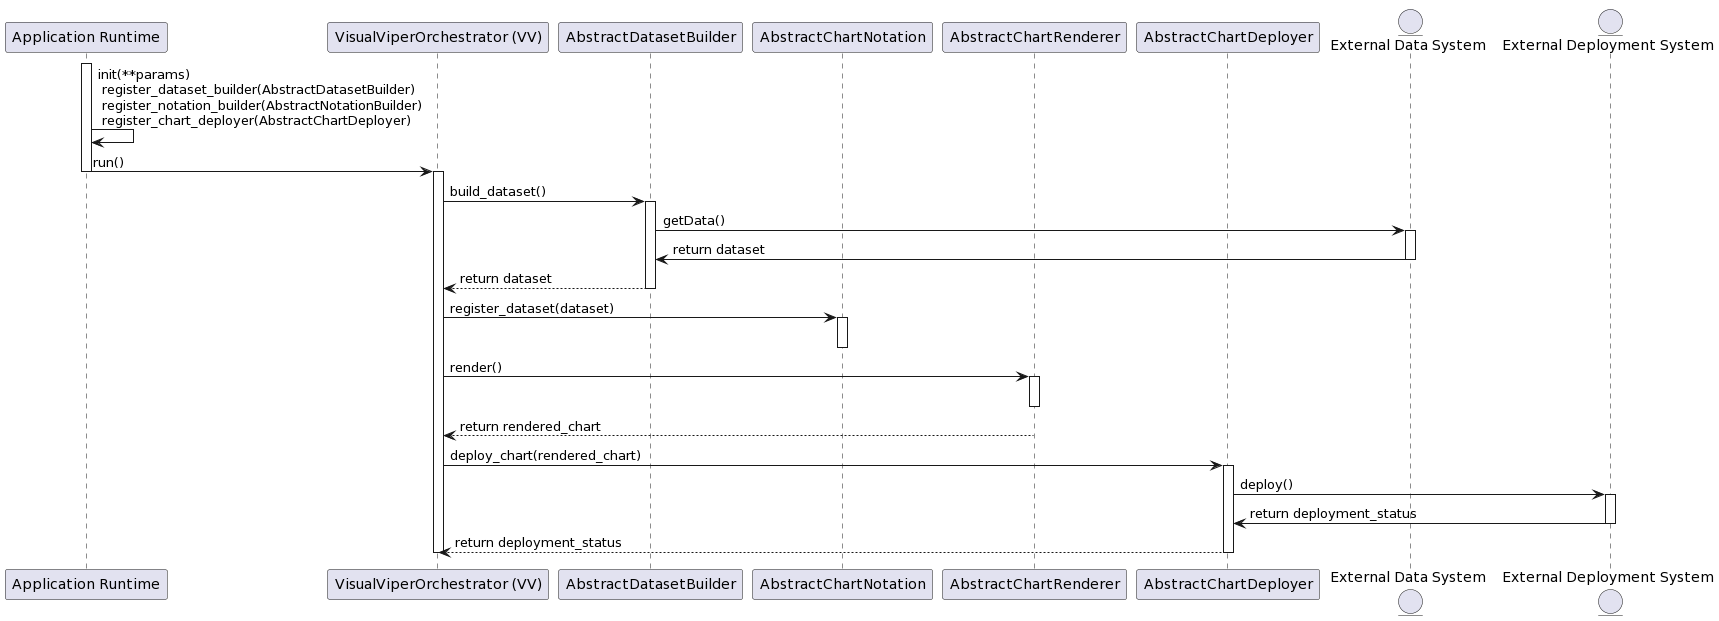
\includegraphics[width=\linewidth]{media/fig9.png}
  \caption{Sequence Diagram for Chart Creation and Deployment in Visual
  Viper Framework.}
  \label{fig:seq_diag}
\end{figure}
\end{landscape}
}

\paragraph{Sequence of Operations}\label{sequence-of-operations}

To provide a more concrete understanding of the interactions between
components, Figure \ref{fig:seq_diag} presents a sequence diagram illustrating the flow
of operations in a typical use case. This diagram was also constructed
using PlantUML.

In this sequence diagram:

\begin{enumerate}
\def\labelenumi{\arabic{enumi}.}
\item
  The Application Runtime initializes the VisualViperOrchestrator and
  registers the required components: AbstractDatasetBuilder,
  AbstractChartNotation, AbstractChartRenderer, and
  AbstractChartDeployer.
\item
  The VisualViperOrchestrator initiates the dataset construction process
  by calling the build\_dataset() method on an AbstractDatasetBuilder
  object. This object may retrieve data from an external system,
  abstracted here for generality.
\item
  Upon successful dataset construction, the VisualViperOrchestrator
  registers the dataset with AbstractChartNotation for further
  processing.
\item
  The VisualViperOrchestrator then invokes the render() method on an
  AbstractChartRenderer object to create the actual visual
  representation.
\item
  Finally, the VisualViperOrchestrator calls the deploy\_chart() method
  on an AbstractChartDeployer object, deploying the rendered chart to an
  external system.
\end{enumerate}

This sequence of operations encapsulates the VV system\textquotesingle s
core functionality while emphasizing its modularity and extensibility.
It serves as an exemplar flow, illustrating how the system components
interact to accomplish the data visualization task.

\section{Description of Components}\label{description-of-components}

In this section, we elaborate on the various components of our system,
their roles, and how they interact. To give you a comprehensive
understanding, we\textquotesingle ve included a directory structure in
Figure \ref{fig:folders}.


\begin{figure}[ht]
  \centering
  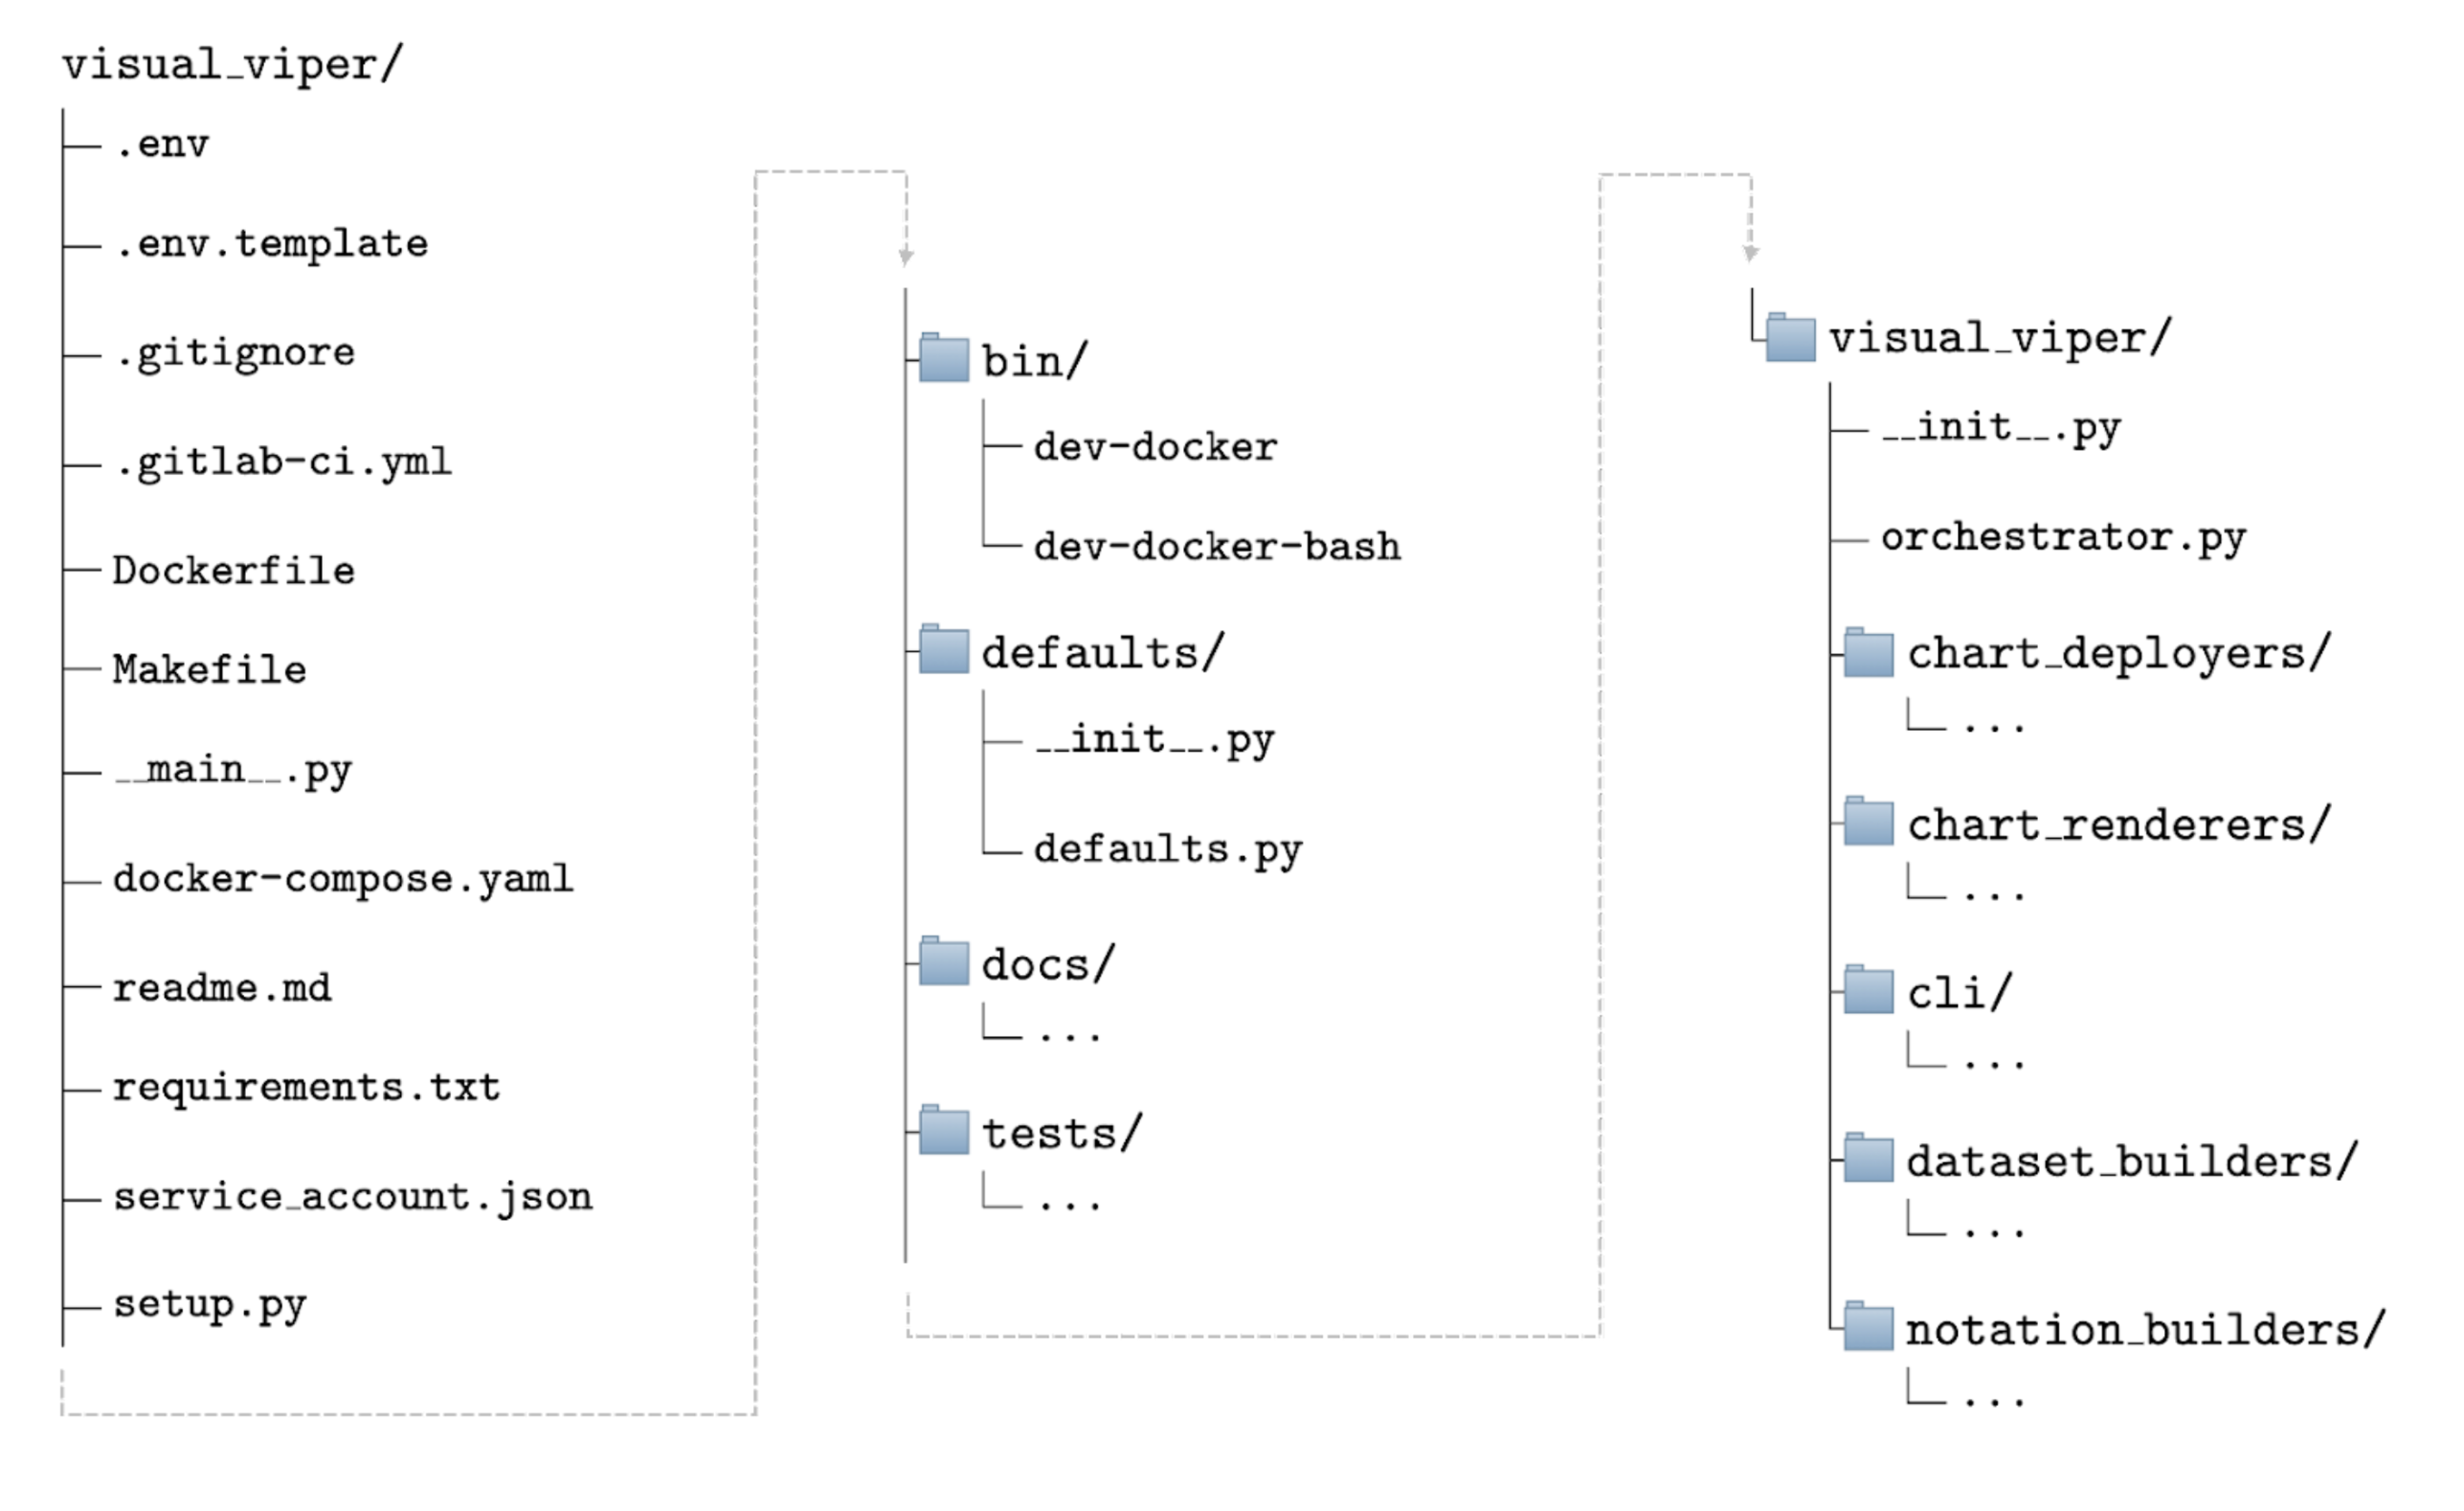
\includegraphics[width=\textwidth]{media/fig10.png}
  \caption{Directory structure of the project. The directory structure
  and the following graphical diagram were generated using
  VV\textquotesingle s directory description and LaTeX diagramming plugins
  (not described in the current work). For brevity, certain folders have
  been excluded or their contents omitted from this diagram.}
  \label{fig:folders}
\end{figure}


\subsection{Key Directories and Their Functional
Roles}\label{key-directories-and-their-functional-roles}

\begin{itemize}
\item
  \textbf{defaults/}: This directory contains the default configuration
  settings, enabling the system to operate with a predefined set of
  parameters.
\item
  \textbf{docs/}: Comprising comprehensive documentation, this directory
  aids in the effective utilization and understanding of the system.
\item
  \textbf{tests/}: This is dedicated to unit testing.
\item
  \textbf{visual\_viper/:} This directory encapsulates the core
  functionalities and classes of the project, which include the
  orchestrators and Command-Line Interface (CLI) mechanisms (which is
  still under development).
\end{itemize}

\subsection{Alignment with Design
Philosophy}\label{alignment-with-design-philosophy}

The directory structure reflects the project's commitment to modularity
and extensibility, design philosophies that are integral to the project.
The clear demarcation of responsibilities through specialized
directories, such as those for dataset builders, notation builders,
chart renderers, and chart deployers, underscores the project's modular
and extensible architecture.

\section{Data Flow among
Components}\label{data-flow-among-components}

To complement the understanding of the system\textquotesingle s
architecture, Figure \ref{fig:data_flow} provides a simplified data flow diagram that
outlines the relationships and interactions among key components. The
diagram was constructed using the DOT language and serves as a
conceptual map for how data is passed and manipulated within the system.

\begin{figure}[ht]
  \centering
  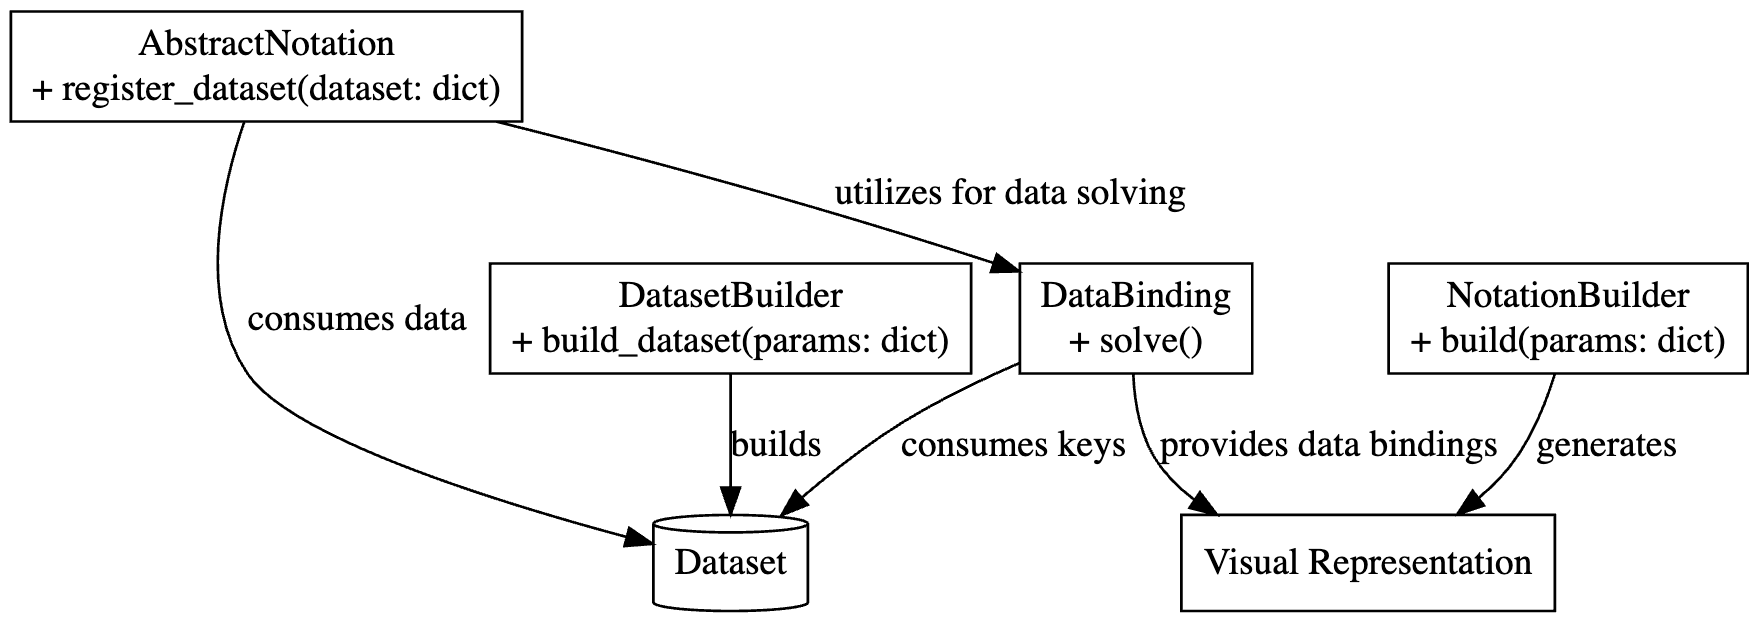
\includegraphics[width=\textwidth]{media/fig11.png}
  \caption{Data Flow Diagram of Key System Components of Visual Viper.}
  \label{fig:data_flow}
\end{figure}

As illustrated in Figure \ref{fig:data_flow}:

\begin{itemize}
\item
  \textbf{DatasetBuilder}: Initiates the process by constructing the
  dataset based on the provided parameters.
\item
  \textbf{Dataset}: Serves as the data store which is consumed by both
  the DataBinding and AbstractNotation classes.
\item
  \textbf{NotationBuilder}: Builds the visual representation of the
  chart, laying out the aesthetics and graphical elements.
\item
  \textbf{Visual Representation}: This is the generated graphical layout
  of the chart, whose appearance is dictated by the NotationBuilder.
\item
  \textbf{DataBinding}: Consumes keys from the Dataset to resolve any
  data dependencies and supplies this resolved data to the visual
  representation.
\item
  \textbf{AbstractNotation}: This class receives data from the Dataset
  and utilizes the DataBinding class to solve for any data-related
  calculations.
\end{itemize}

The DataBinding class plays a crucial role in combining the dataset with
its visual representation, ensuring that the data points are correctly
mapped onto the chart. On the other hand, the AbstractNotation class
establishes the fundamental structure of the chart, including its
underlying logic and computations.

This high-level overview allows for easy plug-and-play of different
dataset builders, data binding mechanisms, and visual representations,
making the system highly modular and extensible.

\section{Modular and Extensible Plugin
Architecture}\label{modular-and-extensible-plugin-architecture}

In line with the system\textquotesingle s commitment to modularity and
extensibility, the architecture of VV features a plugin-based mechanism.
This is a crucial subsystem within the broader architecture that enables
users to enhance or alter the functionality without changing the core
codebase. It facilitates a more dynamic, user-driven ecosystem that
aligns with the project\textquotesingle s design philosophy. Below we
describe the key aspects of this plugin architecture.

\subsection{Initial Phase Plugins}\label{initial-phase-plugins}

In the initial phase of development, we aimed to build a set of plugins
to meet our most immediate data visualization needs. Specifically, we
focused on the following:

\begin{itemize}
\item
  \textbf{Google Spreadsheet Data Fetcher}: This plugin will serve the
  role of a specialized AbstractDatasetBuilder. It will be designed to
  fetch data from Google Spreadsheets, making it easier for users to
  source data without manual intervention.
\item
  \textbf{Vega-Lite Notation Builders}: A group of specialized
  AbstractChartNotation plugins will be developed to create notations
  for Vega-Lite charts. The focus will initially be on generating Forest
  Plots.
\item
  \textbf{Vega-Altair Chart Renderer}: An implementation of
  AbstractChartRenderer, this plugin will use the Vega-Altair library
  for rendering the visual representation of the charts.
\item
  \textbf{Multi-platform Chart Deployers}: To augment the deployment
  capabilities, we aimed to create two deployer plugins:

  \begin{itemize}
  \item
    \textbf{Google Drive Deployer}: Specialized for storing rendered
    image files in Google Drive, making it convenient for users to
    access and share their visualizations.
  \item
    \textbf{Miro Deployer}: Places the generated charts in Miro boards
    with a predefined layout, aiding in the interpretation and
    comparison of the charts.
  \end{itemize}
\end{itemize}

Our plugin architecture is designed for future expansion, both by our
team and external contributors. It allows for:

\begin{itemize}
\item
  \textbf{User Customization}: Users can tailor the software to their
  needs by adding or removing features.
\item
  \textbf{Easy Maintenance}: Since the core code is not altered when
  adding plugins, system updates are more straightforward.
\item
  \textbf{Community Input}: The architecture is open to contributions
  from others, allowing for further enhancements.
\end{itemize}

This architecture supports the previously described low coupling by
allowing independent development and integration of plugins, and high
cohesion by ensuring each plugin is a self-contained, focused unit of
functionality.


\section{Core Classes and their
Responsibilities}\label{core-classes-and-their-responsibilities}

In the following subsections, we will examine each core class to detail
its role and responsibilities in the system architecture.

\subsection{The `dataset\_builders'
Module}\label{the-dataset_builders-module}

The dataset\_builders module serves as the core for data acquisition in
the Visual Viper Framework. This module offers an abstract class,
AbstractDatasetBuilder, designed to be extended for specific data
sourcing implementations. Its design promotes low coupling, making it
easier to integrate new data sources.

\paragraph{The `AbstractDatasetBuilder'
Class}\label{the-abstractdatasetbuilder-class}

The first class in the architecture is AbstractDatasetBuilder, which is
an abstract class acting as a blueprint for all dataset builders. The
class declares a method build\_dataset(params=None), which subclasses
should implement to provide the actual dataset-building functionality
(Listing \ref{listing:3}). This abstract class is crucial in achieving low coupling as
it ensures that other components of the system need not know the
specific dataset builder that will be used.

\begin{code}
  \begin{minted}
    [
    frame=lines,
    framesep=2mm,
    baselinestretch=1.2,
    bgcolor=LightGray,
    linenos,
    breaklines
    ]
    {python}
class AbstractDatasetBuilder:

  @abc.abstractmethod
  def build_dataset(self, params=None):

    raise NotImplementedError()
\end{minted}
\caption{Code snippet showing the AbstractDatasetBuilder class, which provides a method interface for building datasets.}
\label{listing:3}
\end{code}

\paragraph{The `Key' Class}\label{the-key-class}

Within the dataset\_builders module, there\textquotesingle s a simple
but critical class named Key (Listing \ref{listing:4}). This class serves to
encapsulate key-value pairs used for data retrieval. The Key class has
an initializer that takes two arguments: key and an optional src
parameter. Here, key represents the data attribute, while src can be
used to specify the data source.

\begin{code}
  \begin{minted}
    [
    frame=lines,
    framesep=2mm,
    baselinestretch=1.2,
    bgcolor=LightGray,
    linenos
    ]
    {python}
class Key():

  def __init__(self, key, src=None) -> None:
    self.key = key
    self.src = src
  \end{minted}
  \caption{Code snippet showing the Key class used for encapsulating data retrieval attributes.}
  \label{listing:4}
  \end{code}


The utility of the Key class becomes more evident when used in
conjunction with the notation\_builders module, where it plays an
instrumental role in linking dataset attributes to visual elements in a
chart.

\paragraph{The GoogleSpreadsheetDatasetBuilder
Class}\label{the-googlespreadsheetdatasetbuilder-class}

Extending the AbstractDatasetBuilder is the
GoogleSpreadsheetDatasetBuilder class (Listing \ref{listing:5}). This concrete
implementation utilizes the Google Sheets API to fetch data. The class
uses the gspread library and OAuth 2.0 for secure and efficient data
retrieval. One of the significant advantages of this class is its
ability to handle multiple named ranges across multiple worksheets.

\begin{code}
  \begin{minted}
    [
    frame=lines,
    framesep=2mm,
    baselinestretch=1.2,
    bgcolor=LightGray,
    linenos
    ]
    {python}

from google.oauth2 import service_account as sa
from googleapiclient.discovery import build

from .abstract_dataset_builder import *

class GoogleSpreadsheetDatasetBuilder(AbstractDatasetBuilder):

  DEFAULT_SA_PATH = "./service_account.json"
  DEFAULT_SCOPES = ['https://www.googleapis.com/auth/drive']

  def __init__(self, file_id=None, sa_path=None) -> None:
    self.file_id = file_id
    self.sa_path = sa_path or self.DEFAULT_SA_PATH
    self.auth = sa.Credentials.from_service_account_file(
      self.sa_path,
      scopes=self.DEFAULT_SCOPES
    )
    self.dataset = dict()

  def build(self, params=None, ws_index=0):
    gs = gspread.service_account(self.sa_path)
    range_sets = dict()

    for el in params["ranges"]:
      if not isinstance(el, tuple):
        el = (el, self.file_id)
      named_range, file_id = el
      if not file_id in range_sets:
        range_sets[file_id] = []
      range_sets[file_id].append(named_range)

    for file_id, ranges in range_sets.items():
      sheet = gs.open_by_key(file_id)
      worksheet = sheet.get_worksheet(ws_index)
      response = worksheet.batch_get(
        ranges,
        value_render_option="UNFORMATTED_VALUE",
      )
      response = {
        ranges[i]: response[i][0][0] for i in range(len(response))
      }
      self.dataset.update(response)
    return self.dataset

  \end{minted}
  \caption{Code snippet showing the GoogleSpreadsheetDatasetBuilder
  class, responsible for building datasets from Google Sheets.}
  \label{listing:5}
  \end{code}

  \subsection{The `notation\_builders'
Module}\label{the-notation_builders-module}

The notation\_builders module encapsulates the logic required for
constructing the chart notations and solving data dependencies for the
actual visualization. Two abstract classes form the core of this module:
AbstractChartNotationBuilder and AbstractChartNotation.

\paragraph{The `AbstractChartNotationBuilder'
Class}\label{the-abstractchartnotationbuilder-class}

AbstractChartNotationBuilder is an abstract class that acts as a
blueprint for all chart notation builders (Listing \ref{listing:6}). It declares
methods like build() that subclasses need to implement to
provide the actual chart-building functionality. The class uses an
internal property bindings, designed to be overridden in subclasses,
that links the dataset keys to visual elements in a chart.

The AbstractChartNotationBuilder class also introduces a collect\_keys()
method, which traverses all the bindings and collects the Key instances,
serving as a bridge to the dataset\_builders module. This method ensures
that all necessary data points can be fetched efficiently from the
dataset.

\begin{code}
  \begin{minted}
    [
    frame=lines,
    framesep=2mm,
    baselinestretch=1.2,
    bgcolor=LightGray,
    linenos
    ]
    {python}
class AbstractChartNotationBuilder:
  # ...

  def _init_(self, bindings=None, id=None, opts=None):
    # ...

  @property
  def bindings(self):
    raise NotImplementedError()

  def collect_keys(self, dataset):
    # ...

  @abc.abstractmethod
  def build(self, params=None) -> dict:
    raise NotImplementedError()
  \end{minted}
  \caption{Code snippet showing the AbstractChartNotationBuilder class,
  which serves as the framework for building chart notations.}
  \label{listing:6}
  \end{code}

\paragraph{The `AbstractChartNotation'
Class}\label{the-abstractchartnotation-class}

The AbstractChartNotation class functions as a complementary element to
the AbstractChartNotationBuilder class. This class registers the dataset
and contains a solve() method. The solve() method uses instances of the
Key class from the dataset\_builders module to fetch the necessary data
points, thereby linking the chart notation to the actual data (Listing
\ref{listing:7}).

\begin{code}
  \begin{minted}
    [
    frame=lines,
    framesep=2mm,
    baselinestretch=1.2,
    bgcolor=LightGray,
    linenos
    ]
    {python}
class AbstractChartNotation:

  def _init_(self):
    self.dataset = {}

  def register_dataset(self, dataset):
    # ...

  def solve(self, el):
    # ...

  \end{minted}
  \caption{Code snippet showing the AbstractChartNotation class, which
  registers the dataset and provides a method for solving notation
  elements.}
  \label{listing:7}
  \end{code}

\paragraph{The `ForestPlot' Class}\label{the-forestplot-class}


The ForestPlot class (Listing \ref{listing:8}) is a concrete implementation that
inherits from AbstractChartNotationBuilder. It specializes in building
Forest Plots, a type of chart that is commonly used to visualize grouped
data points in a graphical format. The class provides the option to
include labels for different measures (hr, lo, hi) and customizes them
as needed.

\begin{code}
  \begin{minted}
    [
    frame=lines,
    framesep=2mm,
    baselinestretch=1.2,
    bgcolor=LightGray,
    linenos
    ]
    {python}
from .abstract_notation_builder import AbstractChartNotationBuilder
from .forest_plot_binding_notation import ForestPlotBinding

class ForestPlot(AbstractChartNotationBuilder):

  OPTS = dict(
    labels = dict(
      hr="HR",
      lo="CI Low",
      hi="CI High",
    )
  )

  @property
  def bindings(self):
    return [
      ForestPlotBinding(
        measure="",
        hr=self.opts["labels"]["hr"],
        lo=self.opts["labels"]["lo"],
        hi=self.opts["labels"]["hi"],
      ),
      *self._bindings
    ]

  def build(self, params=None) -> dict:
    base_schema = {
      "$schema": "https://vega.github.io/schema/vega-lite/v5.json",
      "data": {
        "values": [
        ]
      },
      #...
    }
    notation = base_schema.copy()
    values = [binding.solved_data for binding in self.bindings]
    notation["data"]["values"] = values
    return notation

  \end{minted}
  \caption{Code snippet showing the ForestPlot class, responsible for
  building the notation for Forest Plots.}
  \label{listing:8}
  \end{code}


The ForestPlot class overrides the bindings property, providing a
default ForestPlotBinding instance that serves as a blueprint for all
bindings related to this specific type of chart. It also defines the
build(params=None) method to generate the notation for rendering the
chart using the Vega-Lite schema.

\paragraph{The ForestPlotBinding
Class}\label{the-forestplotbinding-class}

This class inherits from AbstractChartNotation and serves to hold and
solve the data points necessary for a Forest Plot. Unlike the generic
AbstractChartNotation, ForestPlotBinding has additional properties
specific to Forest Plots, such as hr (Hazard Ratio), lo (Low Confidence
Interval), and hi (High Confidence Interval), as can be seen in Listing
\ref{listing:9}.

The ForestPlotBinding class introduces the data and solved\_data
properties. The data property returns the initial (unsolved) key-value
pairs, whereas the solved\_data property uses the inherited solve()
method to get the actual data points from the dataset. These properties
bridge the gap between data sourcing and data representation in the
chart.

\begin{code}
  \begin{minted}
    [
      frame=lines,
      framesep=2mm,
      baselinestretch=1.2,
      bgcolor=LightGray,
      linenos,
      breaklines
      ]
      {python}
import json
from .abstract_chart_notation import AbstractChartNotation

class ForestPlotBinding(AbstractChartNotation):

  def __init__(self, measure, hr, lo, hi) -> None:
    super().__init__()
    self.measure = measure
    self._hr = hr
    self._lo = lo
    self._hi = hi

  @property
  def data(self) -> dict:
    return dict(
      measure=self.measure,
      lo=self._lo,
      hr=self._hr,
      hi=self._hi,
    )

  @property
  def solved_data(self) -> dict:
    return dict(
      measure=self.measure,
      lo=self.lo,
      hr=self.hr,
      hi=self.hi,
    )

  @property
  def lo(self):
    return self.solve(self._lo)

  @property
  def hr(self):
    return self.solve(self._hr)

  @property
  def hi(self):
    return self.solve(self._hi)

  def items(self):
    yield ("hr", self._hr)
    yield ("lo", self._lo)
    yield ("hi", self._hi)

  def __repr__(self):
    return f"hr:{self.hr}, lo:{self.lo}, hi:{self.hi}"
  \end{minted}
  \caption{Code snippet showing the ForestPlotBinding class, which
  encapsulates the logic for holding and solving data points specific to
  Forest Plots.}
  \label{listing:9}
  \end{code}

\paragraph{Summary Diagram for the `notation\_builders'
Module}\label{summary-diagram-for-the-notation_builders-module}

To sum up the relationships between these classes, please refer to the
following class diagram depicted in Figure \ref{fig:class_diag2}.

\begin{figure}[!ht]
  \centering
  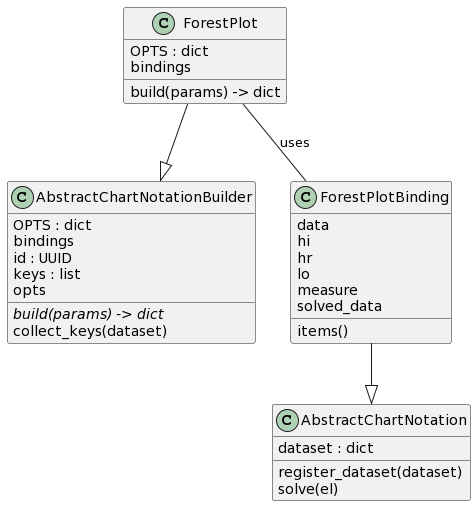
\includegraphics[width=0.5\textwidth]{media/fig12.png}
  \caption{Class diagram of the classes included in the
  `notation\_builders' module.}
  \label{fig:class_diag2}
\end{figure}

The ForestPlot class inherits from AbstractChartNotationBuilder, while
ForestPlotBinding inherits from AbstractChartNotation. The ForestPlot
class uses instances of ForestPlotBinding to build the chart, leveraging
the options and methods provided by the parent classes.

Again, this setup ensures low coupling and high cohesion, thus aligning
well with the principles of clean architecture.

\subsection{The `chart\_renderers'
Module}\label{the-chart_renderers-module}

The chart\_renderers module is a pivotal component in the VV Framework
responsible for rendering visualizations. The module houses an abstract
class, AbstractChartRenderer, which is designed to be extended by
specific rendering engines.

\paragraph{The `AbstractChartRenderer'
Class}\label{the-abstractchartrenderer-class}

The backbone of the chart\_renderers module is the AbstractChartRenderer
class (Listing \ref{listing:10}). It is an abstract class serving as a blueprint for
all chart rendering implementations. It declares a method
render(notation=None, params=None), which is expected to be implemented
by subclasses to provide the actual chart rendering functionality. This
design pattern ensures that other system components do not need to be
aware of the specific renderer in use, thereby achieving low coupling.

\begin{code}
  \begin{minted}
    [
      frame=lines,
      framesep=2mm,
      baselinestretch=1.2,
      bgcolor=LightGray,
      linenos
      ]
      {python}
class AbstractChartRenderer:
  def _init_(self) -> None:
    pass

  def render(self, notation=None, params=None):
    raise NotImplementedError
  \end{minted}
  \caption{Code snippet showing the AbstractChartRenderer class, which
  provides a method interface for rendering charts.}
  \label{listing:10}
  \end{code}

\paragraph{The `AltairChartRenderer'
Class}\label{the-altairchartrenderer-class}

Extending the AbstractChartRenderer is the AltairChartRenderer class
(Listing \ref{listing:11}). This specialized class serves as a wrapper for Vega-Altair,
utilizing the Altair library to perform the rendering of visualizations.
One of its key features is the flexibility of outputting the rendered
chart through a file pointer (fp). This fp can be either a string
representing a file path or an in-memory file-like object such as a
StringIO object. This offers versatility for different use-cases,
including real-time chart generation and embedding charts into web
applications.

By overriding the render method, this class takes in a chart notation
and a file pointer (fp) parameter. The chart is generated from the
notation and saved in SVG format to the location pointed to by fp.

\begin{code}
  \begin{minted}
    [
      frame=lines,
      framesep=2mm,
      baselinestretch=1.2,
      bgcolor=LightGray,
      linenos
      ]
      {python}
import altair
from .abstract_chart_renderer import AbstractChartRenderer

class AltairChartRenderer(AbstractChartRenderer):
  def _init_(self) -> None:
    super().__init__()

  def render(self, fp, notation=None, params=None):
    chart = altair.Chart.from_dict(notation)
    chart.save(fp, format="svg")
    return fp
  \end{minted}
  \caption{Code snippet showing the AltairChartRenderer class, which
  acts as a wrapper for Vega-Altair and is responsible for rendering
  charts using the Altair library.}
\label{listing:11}
\end{code}


\subsection{The `chart\_deployers'
Module}\label{the-chart_deployers-module}

The chart\_deployers module serves as the component in the VV Framework
that specializes in the deployment of visualizations. This module
introduces an abstract class, AbstractChartDeployer, which acts as a
blueprint for various chart deployment strategies, including concrete
implementations like GdriveChartDeployer and MiroChartDeployer. These
implementations provide specialized mechanisms for deploying charts to
Google Drive and Miro boards, respectively. The design of the module
encourages low coupling, allowing easy integration of different
deployment methods without altering the core framework.

\paragraph{The AbstractChartDeployer
Class}\label{the-abstractchartdeployer-class}

The foundational class in this architecture is AbstractChartDeployer, an
abstract class that defines the standard for all chart deployers
(Listing \ref{listing:12}). It declares a method deploy\_chart(buffer, params=None),
which is designed to be overridden by subclasses to offer the actual
chart deployment functionality.

\begin{code}
  \begin{minted}
    [
      frame=lines,
      framesep=2mm,
      baselinestretch=1.2,
      bgcolor=LightGray,
      linenos
      ]
      {python}
class AbstractChartDeployer:

  @abc.abstractmethod
  def deploy_chart(buffer: io.BytesIO, params=None) -> None:
    raise NotImplementedError()
  \end{minted}
  \caption{Code snippet showing the AbstractChartDeployer class, which provides a method interface for deploying charts.}
  \label{listing:12}
  \end{code}

\paragraph{The `GdriveChartDeployer'
Class}\label{the-gdrivechartdeployer-class}

Extending the AbstractChartDeployer is the GdriveChartDeployer class
(Listing \ref{listing:13}). This concrete implementation leverages Google
Drive\textquotesingle s API for the deployment of visualizations. It
uses the google-auth and google-api-python-client libraries for secure
and authenticated communication with Google Drive.

\begin{code}
  \begin{minted}
    [
      frame=lines,
      framesep=2mm,
      baselinestretch=1.2,
      bgcolor=LightGray,
      linenos
      ]
      {python}
class GdriveChartDeployer(AbstractChartDeployer):

  DEFAULT_SA_PATH = "./service_account.json"
  DEFAULT_SCOPES = ['https://www.googleapis.com/auth/drive']
  DEFAULT_FILE_NAME = "filename.svg"

  def __init__(self, folder_id, mime_type=None, sa_path=None, params=None):
    self.sa_path = sa_path or self.DEFAULT_SA_PATH
    self.auth = sa.Credentials.from_service_account_file(
      self.sa_path,
      scopes=self.DEFAULT_SCOPES
    )
    self.drive_service = build('drive', 'v3', credentials=self.auth)
    self.folder_id = folder_id
    self.file_name = params.get("filename") if params else self.DEFAULT_FILE_NAME
    self.mime_type = mime_type

  def deploy(self, fp):
    files = []
    file_metadata = {
      'name': self.file_name,
      'parents': [self.folder_id],
    }

    if hasattr(fp, 'getvalue'):
      content = BytesIO(fp.getvalue().encode("utf-8"))
    elif isinstance(fp, (str, bytes, os.PathLike)):
      with open(fp, 'rb') as file:
        content = file.read()
    else:
      raise TypeError("fp must be a file-like object or a file path")

    #...
    response = request.execute()
    return response.get('id')
  \end{minted}
  \caption{Code snippet showing the GdriveChartDeployer class,
  responsible for deploying charts to Google Drive.}
  \label{listing:13}
  \end{code}

\paragraph{The `MiroChartDeployer'
Class}\label{the-mirochartdeployer-class}

Another subclass of AbstractChartDeployer is the MiroChartDeployer class
(Listing \ref{listing:14}). This specialized class is designed for deploying charts to
Miro boards. It uses Miro\textquotesingle s REST API for communication
with Miro boards.

\begin{code}[ht]
  \begin{minted}
    [
      frame=lines,
      framesep=2mm,
      baselinestretch=1.2,
      bgcolor=LightGray,
      linenos,
      breaklines
      ]
      {python}
class MiroChartDeployer(AbstractChartDeployer):

  DEFAULT_IMAGE_WIDTH = 2000
  DEFAULT_IMAGE_X_POSITION = 0
  DEFAULT_IMAGE_Y_POSITION = 0
  DEFAULT_IMAGE_TITLE = "Default Image Title"

  DEFAULT_LAYOUT_COLUMNS = 2
  DEFAULT_LAYOUT_COLUMN_SPACING = 150
  DEFAULT_LAYOUT_ROW_SPACING = 150

  def __init__(self, board_id, token, params=None):
    self.board_id = board_id
    self.oauth_token = token
    self.parent_id = params.get("parent_id") if params else None

    self.image_title = params.get("image_title") if params else self.DEFAULT_IMAGE_TITLE
    self.image_width = params.get("image_width") if params else self.DEFAULT_IMAGE_WIDTH
    self.image_x_position = params.get("image_x_position") if params else self.DEFAULT_IMAGE_X_POSITION
    self.image_y_position = params.get("image_y_position") if params else self.DEFAULT_IMAGE_Y_POSITION

    self.layout_columns = params.get("layout_columns") if params else self.DEFAULT_LAYOUT_COLUMNS
    self.layout_x_position = params.get("layout_x_position") if params else self.DEFAULT_IMAGE_X_POSITION
    self.layout_row_spacing = params.get("layout_row_spacing") if params else self.DEFAULT_LAYOUT_ROW_SPACING
    self.layout_column_spacing = params.get("layout_column_spacing") if params else self.DEFAULT_LAYOUT_COLUMN_SPACING

    self.deployment_counter = 0
    self.row_elements_height = []
    self.last_widget_id = None

  def calc_position(self, last_widget_id=None):
    # ...

  def get_widget_attribute(self, widget_id, attribute_path):
    # ...

  def deploy(self, fp):
    # ...
  \end{minted}
  \caption{Code snippet showing the MiroChartDeployer class, specialized
  in deploying charts to Miro boards.}
  \label{listing:14}
  \end{code}

The MiroChartDeployer class encapsulates a set of attributes and methods
designed to automate the deployment of charts onto a Miro board. Within
the class, several attributes warrant particular attention for their
role in shaping the class functionality:

\begin{itemize}
\item
  Default Constants: A suite of class-level constants prefixed with
  DEFAULT\_ is defined to establish fallback values for various
  properties.
\item
  deployment\_counter: This attribute serves as a counter of the number
  of deployments executed through the deploy method.
\item
  row\_elements\_height: This list-based attribute is specifically
  designed to capture the height of individual elements within each row
  on the Miro board. The data stored in this list informs the layout
  calculations, facilitating the arrangement of multiple widgets on the
  board.
\item
  last\_widget\_id: After each successful deployment, the ID of the last
  deployed widget is stored in this attribute for later manipulation
  (namely getting the widget height for layout calculations).
\end{itemize}

The deploy(fp) method is responsible for actually uploading a chart as
an image widget onto a Miro board. It accepts the parameter fp, which
stands for file pointer.

The calc\_position method is designed to calculate the position for
placing a new image widget on the Miro board according to the parameters
defined for a given structured layout such as number of columns and
column and row spacing.

The get\_widget\_attribute method serves the purpose of fetching
specific attributes from a widget already deployed on the Miro board. It
takes two parameters: widget\_id, the ID of the widget from which an
attribute needs to be fetched, and attribute\_path, a list describing
the nested keys to reach the target attribute in the
widget\textquotesingle s data structure. It is specifically used to get
the height of the last widget which is essential for determining how
much vertical space a row of widgets will occupy in a structured layout
with multiple rows and columns. Specifically, the height attribute helps
to calculate the next y-coordinate (image\_y\_position) for starting a
new row of widgets.

In the calc\_position method, after each widget deployment, the height
of the last deployed widget is fetched and stored in the
row\_elements\_height list. When it\textquotesingle s time to move to a
new row, i.e., when the number of widgets in the current row equals the
predefined maximum number of columns (layout\_columns), the maximum
height in the row\_elements\_height list is used to calculate the new
y-coordinate.
